\documentclass{beamer}
\usepackage{../../shared/styles/custom}
\usepackage{../../shared/styles/conventions}


%\beamerdefaultoverlayspecification{<+->}
% \newcommand{\data}{\mathcal{D}}
% \newcommand\Item[1][]{%
% 	\ifx\relax#1\relax  \item \else \item[#1] \fi
% 	\abovedisplayskip=0pt\abovedisplayshortskip=0pt~\vspace*{-\baselineskip}}


\graphicspath{ {./SVM/} }

\title{SVM Soft Margin Classification}
\date{\today}
\author{Nipun Batra}
\institute{IIT Gandhinagar}
\begin{document}
	\maketitle
	
{
	\setbeamercolor{background canvas}{bg=}
	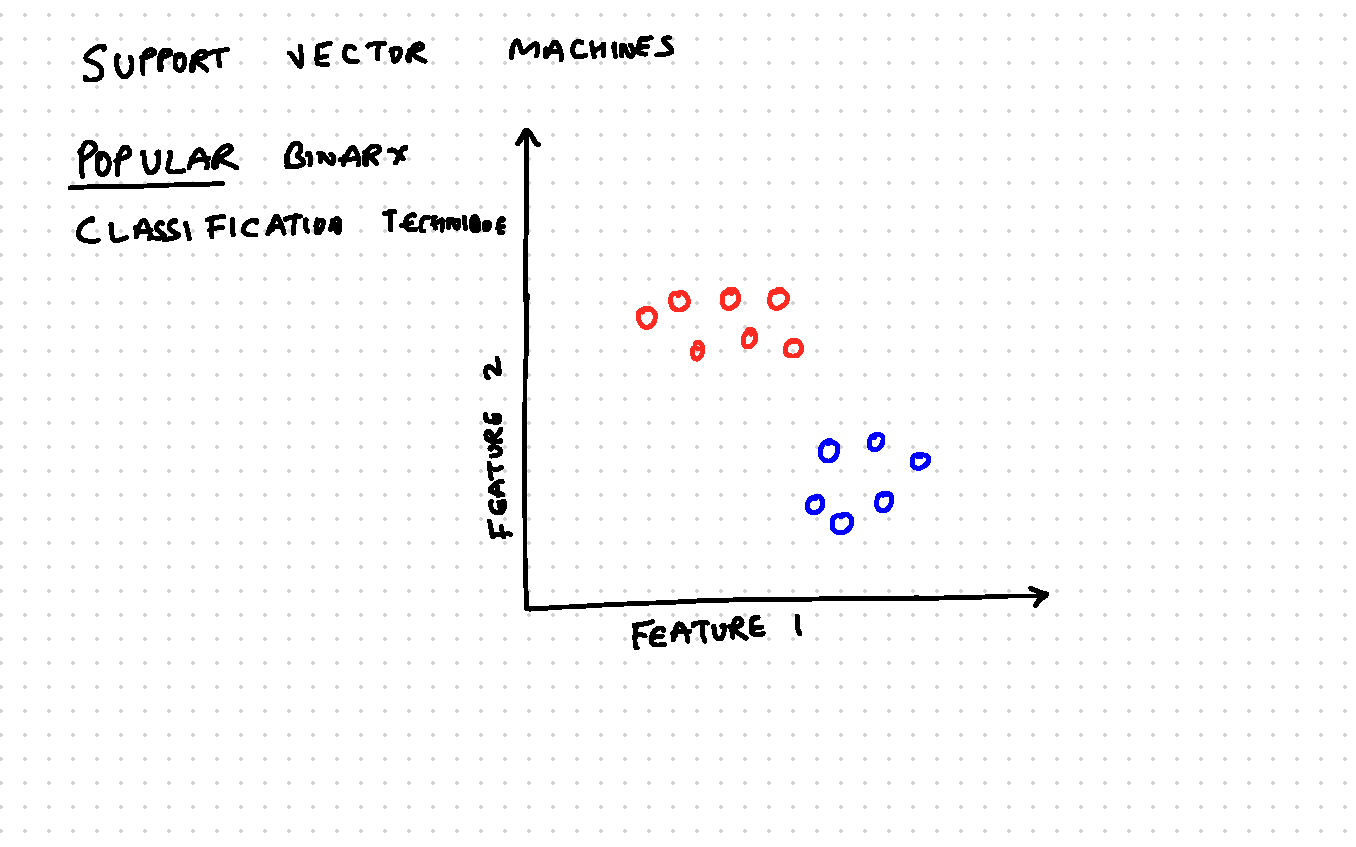
\includepdf[page=50]{Svm-notes.pdf}
}

	
	\begin{frame}{Pop Quiz \#1}
	\begin{tcolorbox}[colback=blue!5!white,colframe=blue!75!black,title=Quick Question!]
	Why might we need a "soft margin" SVM?
	\begin{itemize}
		\item a) Data is perfectly linearly separable
		\item b) Data has some noise and outliers
		\item c) We want smaller margins
		\item d) To avoid using kernels
	\end{itemize}
	\pause
	\textbf{Answer:} b) Data has some noise and outliers - soft margin allows controlled violations.
	\end{tcolorbox}
	\end{frame}

	\begin{frame}{Soft-Margin SVM}
	\begin{itemize}[<+->]
		\item Can we learn SVM for ``slightly'' non-separable data without projecting to a higher space? 
		\item Introduce some ``slack'' ($\xi_i$) or loss or penalty for samples - allow some samples to be misclassified
		
	\end{itemize}
		
		
		
	\end{frame}

{
	\setbeamercolor{background canvas}{bg=}
	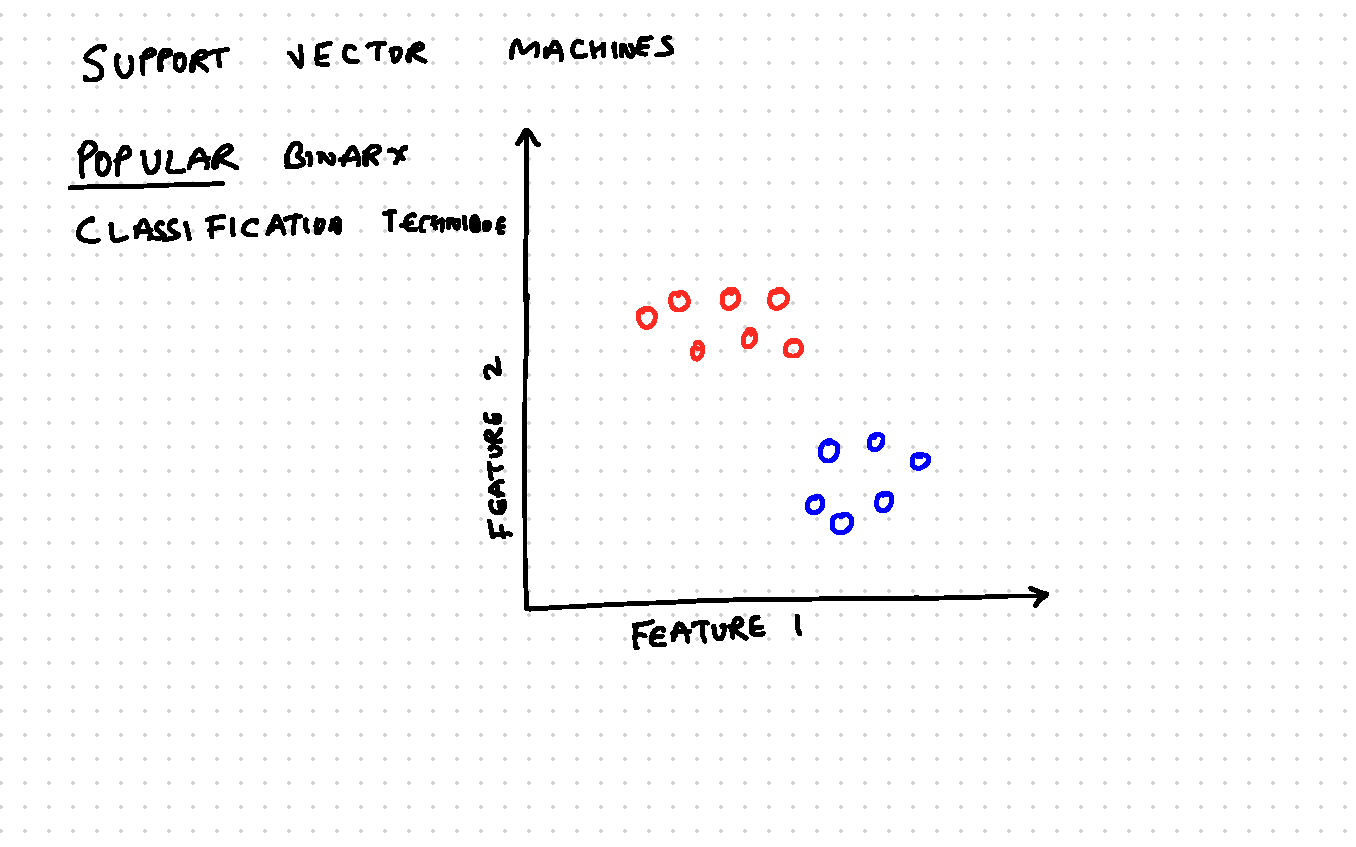
\includepdf[page=51-58]{Svm-notes.pdf}
}
	
	\begin{frame}{Soft-Margin SVM}
		Change Objective \\
		\vspace{0.1cm}
		$\minimize \frac{1}{2}\norm{\vw}^{2} + C \sum_{i=1}^{n}\xi_{i}$ \\ s.t. $y_{i}(\vw \cdot \vx_i + b) \geq 1 - \xi_{i}$ \\
		
		\vspace{0.2cm}
		\pause In Dual:
		$$\minimize \sum_{i=1}^{n}\valpha_{i} - \sum_{i=1}^{n}\sum_{j=1}^{n}\valpha_{i}\valpha_{j}y_{i}y_{j}\vx_{i} \cdot \vx_{j}$$
		s.t.
		$$0 \leq \valpha_{i} \leq C \text{\hspace{0.3cm}\&\hspace{0.3cm}} \sum_{i=1}^{n}\valpha_{i}y_{i} = 0$$
		
	\end{frame}


{
	\setbeamercolor{background canvas}{bg=}
	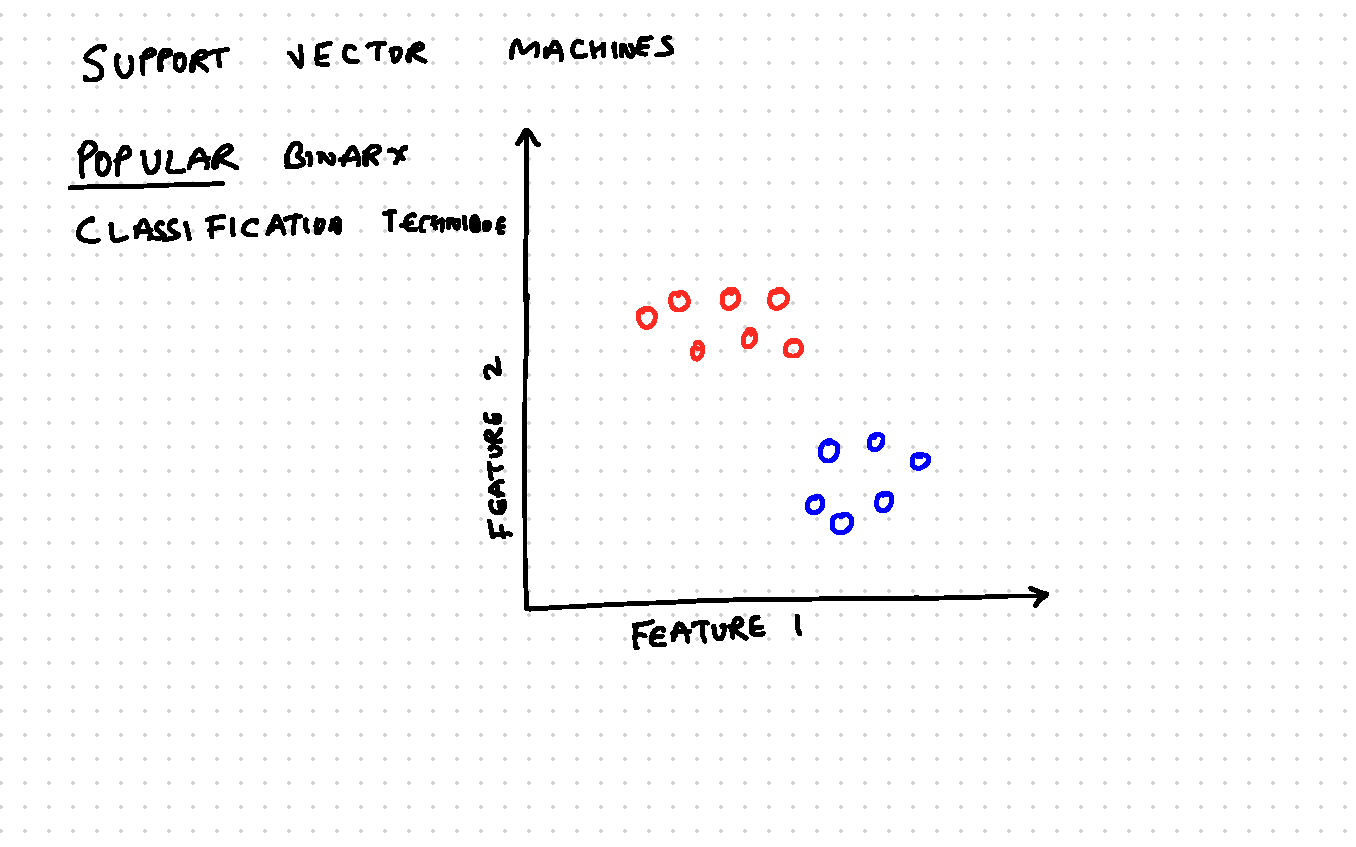
\includepdf[page=59-61]{Svm-notes.pdf}
}

\begin{frame}{Pop Quiz \#2}
\begin{tcolorbox}[colback=blue!5!white,colframe=blue!75!black,title=Quick Question!]
What happens when the regularization parameter $C$ is very large?
\begin{itemize}
	\item a) The model becomes more tolerant to misclassifications
	\item b) The model tries to classify all training points correctly
	\item c) The margin becomes larger
	\item d) Regularization increases
\end{itemize}
\pause
\textbf{Answer:} b) The model tries to classify all training points correctly - high variance!
\end{tcolorbox}
\end{frame}

\begin{frame}{Bias Variance Trade-off for Soft-Margin SVM}
	Low C $\implies$ Higher train error (higher bias) \\
	\vspace{1cm}
	High C $\implies$ Very sensitive to datasete (high variance) \\
\end{frame}

	\begin{frame}{Soft-Margin SVM}
		If C $\rightarrow 0$ \\
		\hspace{0.3cm} Objective $\rightarrow \minimize \frac{1}{2}\norm{\vw}^{2}$ \\
		\hspace{0.3cm} $\implies$ Choose large margin (without worrying for $\xi_{i}$s) \\
		\vspace{0.4cm}
		\hspace{2cm} \framebox{Recall: Margin = $\frac{2}{\norm{\vw}}$}\\
		
		If C $\rightarrow \infty$ (or very large) 
		\hspace{0.3cm} Objective $\rightarrow \minimize C\sum\xi_{i}$ or choose $\vw$, $b$, s.t. $\xi_{i}$ is small!
	\end{frame}
	\begin{frame}{Pop Quiz \#3}
	\begin{tcolorbox}[colback=blue!5!white,colframe=blue!75!black,title=Quick Question!]
	What is the equivalent of hard margin?
	\begin{itemize}
		\item a) C $\rightarrow 0$
		\item b) C $\rightarrow \infty$
	\end{itemize}
	\pause
	\textbf{Answer:} b) C $\rightarrow \infty$ - No violations allowed!
	\end{tcolorbox}
	\end{frame}
	
	\begin{frame}{Pop Quiz \#4}
	\begin{tcolorbox}[colback=blue!5!white,colframe=blue!75!black,title=Quick Question!]
	For a support vector with slack variable $\xi_i = 1.5$, this point is:
	\begin{itemize}
		\item a) On the margin boundary
		\item b) Correctly classified but within margin
		\item c) Misclassified
		\item d) Outside both margins
	\end{itemize}
	\pause
	\textbf{Answer:} c) Misclassified - since $\xi_i > 1$!
	\end{tcolorbox}
	\end{frame}

	\begin{frame}{Soft-Margin SVM}
		Types of support vectors:
		\begin{itemize}
			\item Zone 2: $y_{i}(\vw \cdot \vx_{i} + b) = 1$
			\item Zone 3: $0 < \xi_{i} < 1$ (correctly classified)
			\item Zone 4: $\xi_{i} > 1$ (Misclassified)
		\end{itemize}
		$\therefore$ As C increases, \# support vectors decreases \\
		\vspace{1cm}
		Notebook: SVM-soft-margin
	\end{frame}
	\begin{frame}{SVM Formulation in the Loss + Penalty Form}
		Objective:
		$$\minimize \frac{1}{2}\norm{\vw}^{2} + C\sum_{i=1}^{N}\xi_{i}$$
		Now:
		$$y_{i}(\vw \cdot \vx_{i} + b) \geq 1 - \xi_{i}$$
		$$\xi_{i} \geq 1 - y_{i}(\vw \cdot \vx_{i} + b)$$
		But $\xi_{i} \geq 0$ \\
		$$\therefore \xi_{i} = \max \big[0, 1 - y_{i}(\vw \cdot \vx_{i} + b)\big]$$
	\end{frame}
	\begin{frame}{Pop Quiz \#5}
	\begin{tcolorbox}[colback=blue!5!white,colframe=blue!75!black,title=Quick Question!]
	The hinge loss function $\max[0, 1-y_i(\vw \cdot \vx_i + b)]$ is:
	\begin{itemize}
		\item a) Convex and differentiable everywhere
		\item b) Convex but not differentiable at one point
		\item c) Non-convex but differentiable
		\item d) Neither convex nor differentiable
	\end{itemize}
	\pause
	\textbf{Answer:} b) Convex but not differentiable at $y_i(\vw \cdot \vx_i + b) = 1$!
	\end{tcolorbox}
	\end{frame}

	\begin{frame}{SVM Formulation in the Loss + Penalty Form}
		$\therefore$ Objective is:
		$$\minimize C \sum \xi_{i} + \frac{1}{2}\norm{\vw}^{2}$$
		$$\implies \minimize C \sum_{i=1}^{N} \max\big[0, 1 - y_{i}(\vw \cdot \vx_{i} + b)\big] + \frac{1}{2}\norm{\vw}^{2}$$
		$$\implies \minimize \underbrace{\sum_{i=1}^{N}\max \big[0, 1-y_{i}(\vw \cdot \vx_{i} + b)\big]}_\text{Loss} + \underbrace{ \frac{1}{2C}\norm{\vw}^{2}}_\text{Regularisation}$$
	\end{frame}
	

{
	\setbeamercolor{background canvas}{bg=}
	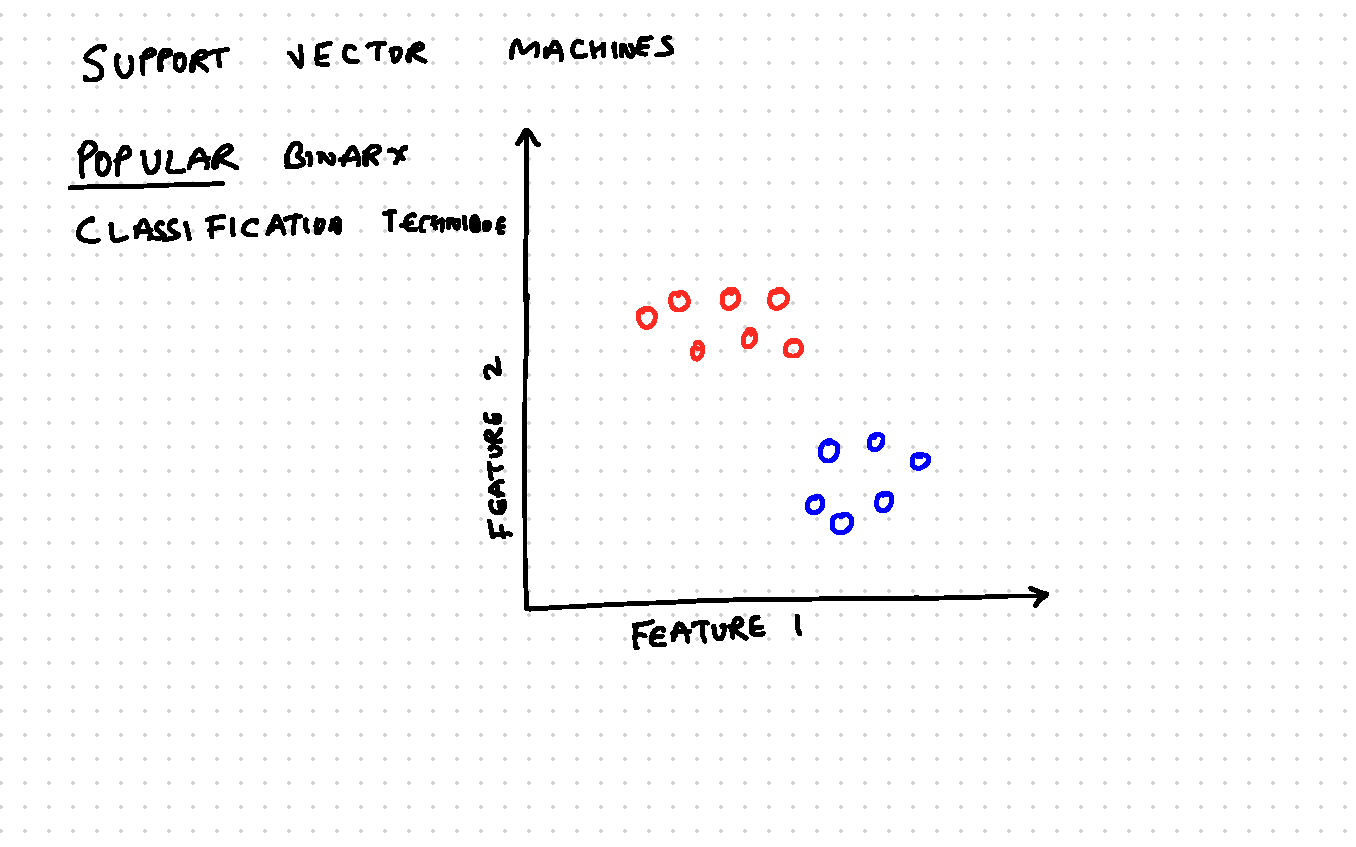
\includepdf[page=62]{Svm-notes.pdf}
}

	\begin{frame}{Loss Function for Sum (Hinge Loss)}
		Loss function is $\sum_{i=1}^{N}\max\big[0, 1 - y_{i}(\vw \cdot \vx_{i} + b)\big]$ \\
		\begin{itemize}[<+->]
			\item Case I 
			\hspace{0.5cm} $y_{i}(\vw \cdot \vx_{i} + b) = 1$ \\
			
			Lies on Margin: $Loss_{i}$ = 0 \\
		
			\item Case II \\
			\hspace{0.5cm} $y_{i}(\vw \cdot \vx_{i} + b) > 1$ \\
			$Loss_{i} = 0$ \\ 
			
			\item 	Case III \\
			\hspace{0.5cm} $y_{i}(\vw \cdot \vx_{i} + b) < 1$ \\
			$Loss_{i} \neq 0$
		\end{itemize}
		
		
	
	\end{frame}
	\begin{frame}{Hinge Loss Continued}
		Q) Is hinge loss convex and differentiable? \\
		\hspace{0.5cm}Convex: $\checkmark$ \\
		\hspace{0.5cm}Differentiable: X\\
		\hspace{0.5cm}Subgradient: $\checkmark$
	\end{frame}
	\begin{frame}{SVM Loss is Convex}
		
		Hinge Loss $\sum(\max[0, (1-y_{i}(\vw \cdot \vx_{i}+b))]$ is convex \\
		\vspace{1cm}
		Penalty $\frac{1}{2}\norm{\vw}^{2}$ is convex \\
		\vspace{1cm}
		$\therefore$ SVM loss is convex
	\end{frame}
	
\end{document}
